
\section{Superfícies}

\subsection*{Cilindros}
%%%%%%%%%%%%%%%%%%%%%%%%%%%%%%%%%%%%%%%%%%%%%%%%%%%%%%%%%%%%%
\begin{frame}[label=cilindros]{Superfícies Cilíndricas}
Uma \dt{superfície cilíndrica} é aquela gerada por uma reta $\ell$ que se move ao longo de uma curva plana dada, de modo que a reta $\ell$ sempre esteja paralela a uma reta fixa. A reta $\ell$ é chada de \dt{geratriz} e a curva de \dt{diretriz}.

\begin{exe}
A equação $z=x^2$ em $\R^3$ representa a seguinte superfície cilíndrica.

\begin{center}
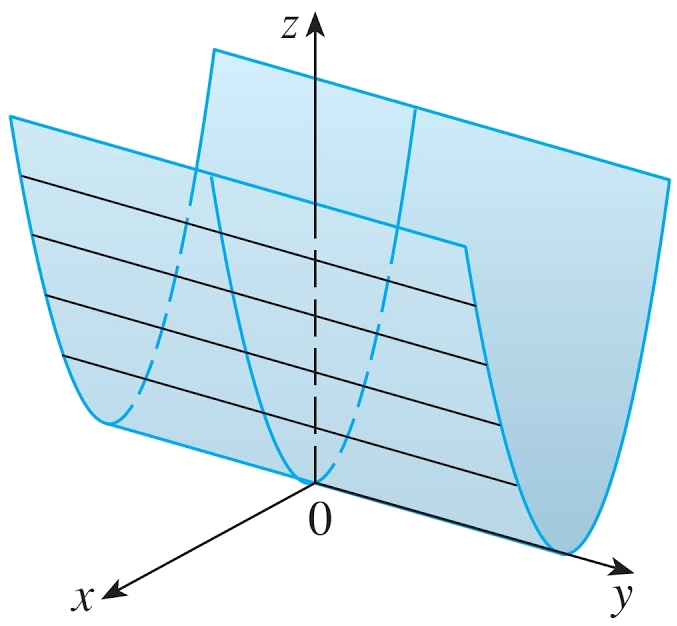
\includegraphics[scale=0.5]{figuras/cilindro-ex1.png}
\end{center}
\end{exe}
\end{frame}

%%%%%%%%%%%%%%%%%%%%%%%%%%%%%%%%%%%%%%%%%%%%%%%%%%%%%%%%%%%%%
\begin{frame}[label=cilindros]{Superfícies Cilíndricas}
\begin{exe}

%\begin{enumerate}
Esboce as superfícies
\begin{enumerate}[a]
\item $y^2+z^2=1$
\item $z=1-y^2$
\end{enumerate}

%\item Determine uma equação para a superfície cilíndrica cuja \dt{diretriz} é o círculo unitário centrado na origem e cujas \dt{geratrizes} são paralelas à reta $r: (x,y,z)=(-t,0,t),\ t\in \R$.
%
%\begin{scriptsize}
%\textbf{Dica:} Note que os pontos dessa superfície são formados pelos círculos unitário centrados na reta $r$.
%\end{scriptsize}
%\end{enumerate}
\end{exe}

\end{frame}
%%%%%%%%%%%%%%%%%%%%%%%%%%%%%%%%%%%%%%%%%%%%%%%%%%%%%%%

\subsection*{Quádricas}


%%%%%%%%%%%%%%%%%%%%%%%%%%%%%%%%%%%%%%%%%%%%%%%%%%%%%%%%%%%%%
\begin{frame}[label=cilindros]{Superfícies Quádricas}
Uma \dt{superfície quádrica} é o gráfico de uma equação do segundo grau a três variáveis, isto é, uma equação da forma:
\begin{equation*}
{\color{red}A}x^2+{\color{red}B}y^2+{\color{red}C}x^2+{\color{red}D}xy
+{\color{red}E}xz+{\color{red}F}yz+{\color{red}G}x+{\color{red}H}y+
{\color{red}I}z+{\color{red}J}=0,
\end{equation*}
onde pelo menos um dos coeficientes ${\color{red}A}, {\color{red}B}, 
{\color{red}C}, {\color{red}D}, {\color{red}E}$ ou ${\color{red}F}$ é não nulo.

\begin{minipage}{0.5\textwidth}
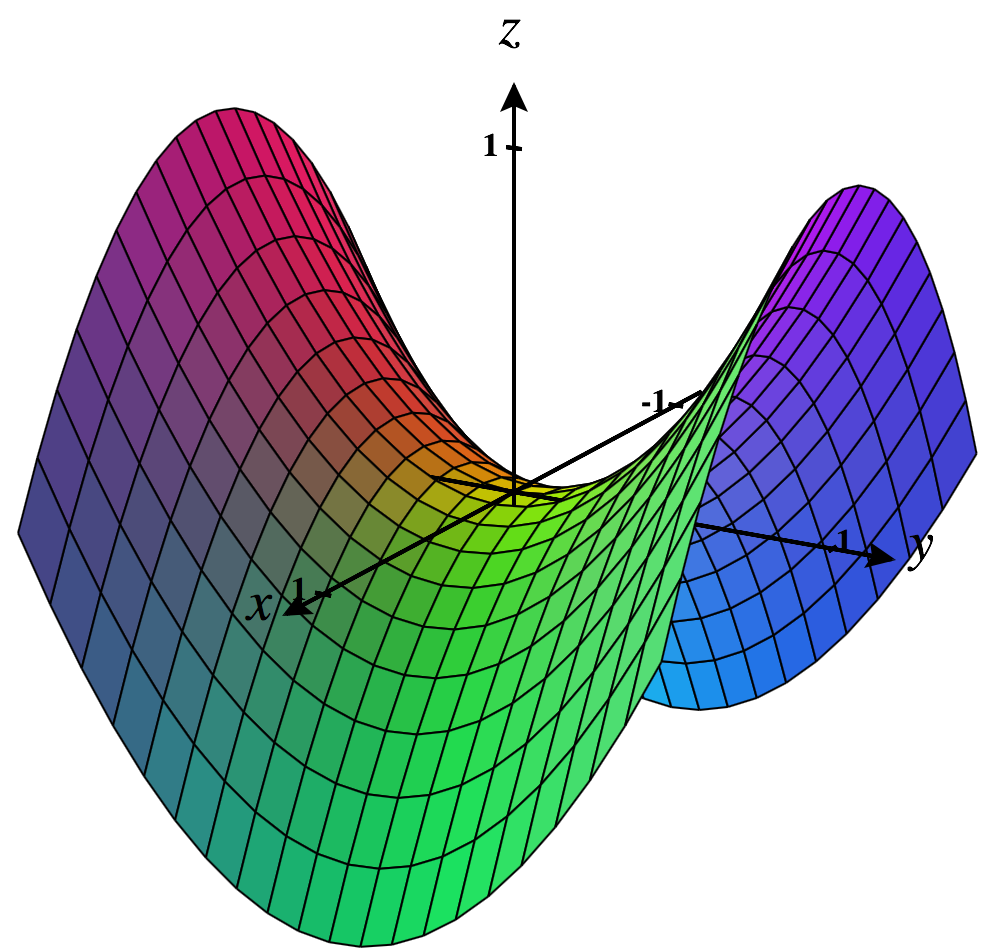
\includegraphics[scale=0.13]{figuras/quadricas/parab-hip.png}
\end{minipage}
\begin{minipage}{0.4\textwidth}
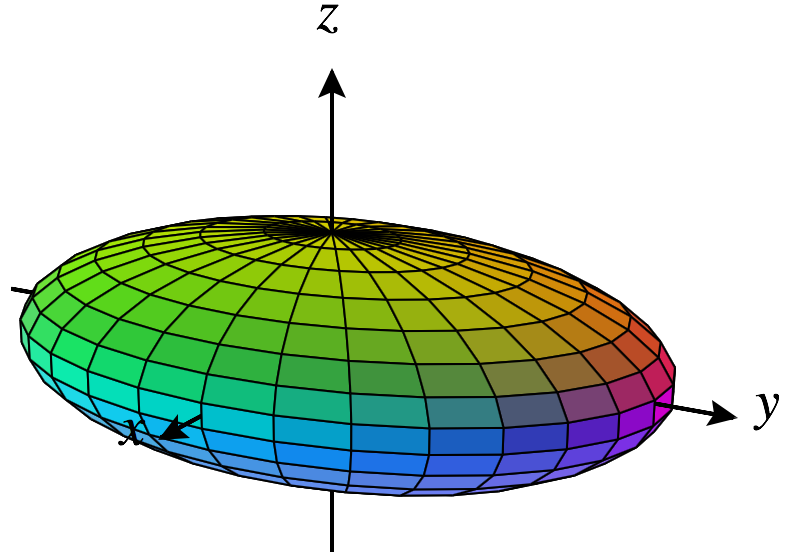
\includegraphics[scale=0.8]{figuras/quadricas/elipsoide.png}
\end{minipage}

\end{frame}
%%%%%%%%%%%%%%%%%%%%%%%%%%%%%%%%%%%%%%%%%%%%%%%%%%%%%%%